\chapter{Theoretical Framework}\label{chap:theory}

\begin{itemize}
  \item Introduce sm
  \item brief history
  \item current areas of study
  \item Reference relevenace to rest of thesis (studying hbb)
\end{itemize}

The Standard Model (SM) of particle physics is the theory describing all known elementary particles and their interactions via three of the four fundamental forces.
Developed by merging the successful theories of quantum mechanics and relativity in the second half of the 20th century, the SM's position today at the centre of our understanding of the nature of the universe is firmly established by an unparalleled level of agreement between the predictions from the model and experimental results \cite{morel2020determination,sailer2022measurement}.

The SM has predicted the discovery of the top and bottom quarks \cite{CDF:1995wbb,D0:1995jca,Herb:1977ek}, the \Wboson and \Zboson bosons \cite{UA1:1983crd}, and the tau neutrino \cite{DONUT:2000fbd}.
The last missing piece of the SM to be discovered was the Higgs boson, first theorised in the 1960s \cite{Englert:1964et,Higgs:1964pj,Guralnik:1964eu}, and eventually observed at the LHC in 2012 \cite{HIGG-2012-27,CMS-HIG-12-028}.
After its discovery, much ongoing work has been carried out performing detailed measurements of its mass and interactions with other particles.

This thesis describes research to improve Higgs analysis to b quarks, by improving algorithm methods\dots


\section{The Standard Model}\label{sec:standard_model}

The SM is formulated in the language of Quantum Field Theory (QFT).
In this framework, particles are localised excitations of corresponding quantum fields, which are operator-valued distribution across spacetime.

Central to QFT is the Lagrangian density which describes the kinematics and dynamics of a field.
Observations of conserved quantities are linked, via Noether's theorem, to symmetries which are expressed by the Lagrangian.
Alongside Global Poincar\'e symmetry, the SM Lagrangian observes a local non-Abelian $SU(3)_C \otimes SU(2)_L \otimes U(1)_Y$ gauge symmetry.
Gauge symmetries leave observable properties of the system unchanged when certain gauge transformations are applied to the fields.
The full Lagrangain of the SM can be broken up into distinct terms corresponding to the different sectors.
An overview of each sector is given in the following chapters.
%
\begin{equation}\label{eq:sm_lagrangian}
  \mathcal{L}_{\textnormal{SM}} = \mathcal{L}_{\textnormal{EW}} + \mathcal{L}_{\textnormal{QCD}} + \mathcal{L}_{\textnormal{Higgs}} + \mathcal{L}_{\textnormal{Yukawa}}
\end{equation}
%
The SM provides a mathematical description of how the four fundamental forces interact with the matter content of the universe.
The SM contains $12$ \spinhalf fermions, listed in \cref{tab:sm_fermions}, and $5$ bosons listed in \cref{tab:sm_bosons}.
%
\begin{table}[!htbp]
  \footnotesize\centering
  \setlength{\tabcolsep}{0.5em} % for the horizontal padding
  \begin{tabular}{c|ccc|ccc}
      \toprule 
      \multicolumn{1}{c|}{} & \multicolumn{3}{c|}{Leptons} & \multicolumn{3}{c}{Quarks} \\
      \hline
      \textbf{Generation} & \textbf{Flavour} & \textbf{Mass} [\unit\MeV] & \textbf{Charge} [\unit\elementarycharge] & 
                            \textbf{Flavour} & \textbf{Mass} [\unit\MeV] & \textbf{Charge} [\unit\elementarycharge] \\
      \hline
      \multirow{2}{*}{First} & 
        $e$        & $0.511$               & -1 & $u$ & $2.16$ & \nicefrac{2}{3} \\
      & $\nu_e$    & $<1.1 \times 10^{-6}$ &  0 & $d$ & $4.67$ & \nicefrac{-1}{3} \\
      %
      \hline
      \multirow{2}{*}{Second} & 
        $\mu$      & $105.7$ & -1 & $c$ & $1.27 \times 10^{3}$ & \nicefrac{2}{3} \\
      & $\nu_\mu$  & $<0.19$ &  0 & $s$ & $93.4$               & \nicefrac{-1}{3} \\
      %
      \hline
      \multirow{2}{*}{Third} & 
        $\tau$     & $1776.9$& -1 & $t$ & $173 \times 10^{3} $ & \nicefrac{2}{3} \\
      & $\nu_\tau$ & $<18.2$ &  0 & $b$ & $4.18  \times 10^{3} $ & \nicefrac{-1}{3} \\
      \bottomrule
  \end{tabular}
  \caption{
    The half-integer spin fermions of the SM \cite{Workman:2022ynf}.
    Three generations of particles are present.
    Also present (unlisted) are the antiparticles, which are identical to the particles up to a reversed charge sign.
    }
  \label{tab:sm_fermions}
\end{table}
%

%
\begin{table}[!htbp]
  \footnotesize\centering
  \setlength{\tabcolsep}{0.5em} % for the horizontal padding
  \begin{tabular}{lcccc}
      \toprule 
      \textbf{Name} & \textbf{Symbol} & \textbf{Mass} [\unit\GeV] & \textbf{Charge} [\unit\elementarycharge] & \textbf{Spin} \\
      \hline
      Photon      & \photon   & $< 1 \times 10^{-27}$     & $< 1 \times 10^{-46}$      & 1    \\
      Weak boson  & \Wpm      & $80.377 \pm 0.012$     & $\pm 1$    & 1    \\
      Weak boson  & \Zboson   & $91.1876 \pm 0.0021$     & 0    & 1    \\
      Gluon       & \gluon    & 0     & 0    & 1    \\
      Higgs       & \higgs    & $125.25 \pm  0.17$     & 0    & 0    \\
      \bottomrule
  \end{tabular}
  \caption{
    The integer spin bosons of the SM \cite{Workman:2022ynf}.
    The photon, weak bosons and gluons are gauge bosons arising from gauge symmetries, and carry the four fundamental forces of the SM.
  }
  \label{tab:sm_bosons}
\end{table}
%
\begin{comment}
  In quantum physics and chemistry, quantum numbers describe values of conserved quantities in the dynamics of a quantum system. Quantum numbers correspond to eigenvalues of operators that commute with the Hamiltonian—quantities that can be known with precision at the same time as the system's energy[note 1]—and their corresponding eigenspaces. Together, a specification of all of the quantum numbers of a quantum system fully characterize a basis state of the system, and can in principle be measured together.
\end{comment}







\subsection{Quantum Electrodynamics}\label{sec:qed}

Consider a Dirac spinor field $\psi = \psi(x)$ and its adjoint $\overline{\psi} = \psi^\dagger \gamma^0$, where $\psi^\dagger$ denotes the Hermitian conjugate of $\psi$.
The field $\psi$ describes fermionic \spinhalf particle, for example an electron.
The Dirac Lagrangian density is
%
\begin{equation}\label{eq:dirac_lagrangian}
  \mathcal{L}_{\textnormal{Dirac}} = \overline{\psi} (i \slashed{\partial}  - m )\psi,
\end{equation}
%
where $\slashed{\partial} = \gamma^\mu \partial_\mu$ denotes the contraction with the Dirac gamma matrices $\gamma^\mu$ (summation over up-down pairs of indices is assumed).
Application of the Euler-Lagrange equation on \cref{eq:dirac_lagrangian} yields the Dirac equation\todo{mention EoMs?}
%
\begin{equation}\label{eq:dirac_eq}
  (i \slashed{\partial}  - m )\psi = 0 .
\end{equation}
%
Suppose some fundamental symmetry that requires invariance under a local $U(1)$ gauge transformation
%
\begin{equation}\label{eq:U(1)_transformation}
  \psi \rightarrow \psi' = \psi e^{- i q \alpha(x)} ,
\end{equation}
%
where $\alpha$ varies over every spacetime point $x$.
Under this transformation, the Dirac equation transforms as 
%
\begin{equation}\label{eq:dirac_eq_transformed}
  (i \slashed{\partial} - m ) \psi e^{- i q \alpha(x)} + q \slashed{\partial}\alpha(x) \psi e^{- i q \alpha(x)} = 0.
\end{equation}
%
For the Dirac equation to remain invariant under the transformation in \cref{eq:U(1)_transformation}, a new field $A_\mu$ which transforms as $A_\mu \rightarrow A'_\mu = A_\mu + \partial_\mu \alpha(x)$ must be added \todo{check consistency with Y=1/2 used later}.
The transformed interaction term
%
\begin{equation}
  - q \slashed{A} \psi \rightarrow - q \slashed{A} \psi e^{- i q \alpha(x)} - q \slashed{\partial} \alpha(x) \psi e^{- i q \alpha(x)}
\end{equation}
%
will then cancel the asymmetric term in \cref{eq:dirac_eq_transformed} as required.
The $U(1)$ invariant Lagrangain can therefore be constructed by adding an interaction between $\psi$ and $A_\mu$ to \cref{eq:dirac_lagrangian}. The kinetic term for the the new field $A_\mu$ is also added in terms of $F_{\mu\nu} = \partial_\mu A_\nu - \partial_\nu A_\mu$, which is trivially invariant under the transformation in \cref{eq:U(1)_transformation}.
The interaction term is absorbed into the covariant derivative $D_\mu = \partial_\mu + i q A_\mu$, thus named as it transforms in the same way as the field $\psi$.
This yields the QED Lagrangain
%
\begin{equation}\label{eq:qed_lagrangian}
  \mathcal{L}_{\textnormal{QED}} = -\frac{1}{4} F_{\mu\nu} F^{\mu\nu} + \overline{\psi} (i \slashed{D} - m )\psi ,
\end{equation}
%
A quadratic term $A_\mu A^\mu$ is not invariant and therefore the the field $A_\mu$ must be massless.
Requiring invariance under local $U(1)$ gauge transformations necessitated the addition of a new field $A_\mu$, corresponding to photons, which interact with charged matter. \todo{improve interpretation}








\subsection{Quantum Chromodynamics}\label{sec:qcd}

Quantum Chromodynamics (QCD) is the study of quarks, gluons and their interactions.
Quarks and gluons carry colour charge, which comes in three kinds, called red, green and blue.
While the $U(1)$ symmetry group in \cref{sec:qed} was Abelian, the QCD Lagrangian is specified by requiring invariance under transformations from the non-Abelian $SU(3)$ group, making it a Yang\nobreakdash-Mills theory \cite{PhysRev.96.191} which requires the addition of self-interacting gauge fields.
The infinitesimal $SU(3)$ group generators are given by $T_a = \lambda_a / 2$, where $\lambda_a$ are the eight Gell\nobreakdash-Mann matrices.
These span the space of infinitesimal group transformations and do not commute with each other, instead satisfying the commutation relation
%
\begin{equation}
  \com{T_a}{T_b} = i f_{abc} T_c ,
\end{equation}
%
where $f_{abc}$ are the group's structure constants.
Consider the six quark fields $q_k = q_k(x)$.
Each flavour of quark $q_k$ transforms in the fundamental triplet representation, where each component of the triplet corresponds to a different value of the colour quantum number.
$G^{a}_{\mu\nu}$ are the eight gluon field strength tensors, one for each generator $T_a$, defined as
%
\begin{equation}\label{eq:qcd_field_strength_tensor}
  G^a_{\mu\nu} = \partial_\mu A_\nu - \partial_\nu A_\mu - g_s f^{abc} A_\mu^b A_\nu^c ,
\end{equation}
%
where $A_\mu^a$ are the gluon fields and $g_s$ is the strong coupling constant. The covariant derivative is written as
%
\begin{equation}\label{eq:qcd_covariant_derivative}
  D_\mu = \partial_\mu + i g_s T_a A_\mu^a .
\end{equation}
%
The full QCD Lagrangain is then given by
%
\begin{equation}\label{eq:qcd_lagrangian}
  \mathcal{L}_\textnormal{QCD} = 
  - \frac{1}{4} G^{a}_{\mu\nu} G_{a}^{\mu\nu}
  + q_k (i \slashed{D} - m_k) q_k .
\end{equation}
%
Cubic and quartic terms of the gauge fields $A^a_\mu$ appear in the Lagrangian, leading to the gluon's self interaction.

The QCD coupling constant $g_s$ varies, or ``runs'', with energy.
At lower energy scales (and corresponding larger distance scales) the interaction is strong.
This leads to quark confinement, whereby an attempt to isolate individual colour-charged quarks requires so much energy that additional quark-antiquark are produced.
At higher energy scales (and corresponding smaller distance scales), asymptotic freedom occurs as the interactions become weaker, allowing perturbative calculations to be performned.
Hadrons are bound states of quarks.
They are invariant under $SU(3)$ gauge transformations (i.e. are colour-charge neutral, or colourless).






\subsection{The Electroweak Sector}\label{sec:ew_sector}

The weak and electromagnetic forces are unified in the Glashow-Weinberg-Salam (GWS) model of electroweak interaction \cite{Glashow:1961tr,Weinberg:1967tq,Salam:1968rm}.
The Lagrangain is specified by requiring invariance under the symmetry group $SU(2)_L \otimes U(1)_Y$, as motivated by a large amount of experimental data.
Here, $SU(2)_L$ is referred to as weak isospin and $U(1)_Y$ as weak hypercharge. (the product of the isospin and hypercharge groups.).

The generators of $SU(2)_L$ are $T_a = \sigma_a/2$, where $\sigma_a$ are the three Pauli spin matrices which satisfy the commutation relation 
%
\begin{equation}
\com{T_a}{T_b} = i \varepsilon_{abc} T_c .
\end{equation}
%
The generator of $U(1)_Y$ is $Y = 1/2$.
Each generator corresponds to a gauge field, which, after symmetry breaking (discussed in \cref{sec:sm_higgs}), give rise to the massive vector bosons, \Wpm and \Zboson, and the massless photon.
The massive vector bosons are the carriers of the weak force, and are unique to the weak sector.
Due to the mass of the force carriers, the weak force has a short range and so it appears weak even though its intrinsic strength is comparable to that of QED.
The gauge bosons acquire mass through the Higgs mechanism, discussed in \cref{sec:sm_higgs}.
\todo{why not mass by hand?}

The weak force violates parity conservation \cite{PhysRev.104.254,PhysRev.105.1413,PhysRev.105.1415}, i.e. invariance under parity transformations (mirror reflections).
Only left handed fermions participate in the weak interaction.
There are no right handed neutrinos in the standard model.
\todo{add parity operator?}
%The Standard Model incorporates parity violation by expressing the weak interaction as a chiral gauge interaction. Only the left-handed components of particles and right-handed components of antiparticles participate in weak interactions in the Standard Model. The weak force couples only to left handed particles in currents of the form $J^\mu = \overline{\nu}_e \gamma^\mu (1 - \gamma^5) e$ or $J^\mu = \overline{u} \gamma^\mu (1 - \gamma^5) \tilde{d}$. The $\tilde{d}$ state is due to the quark mixing: mass eigenstates are not the same as weak eigenstates.
Furthermore, the weak sector exhibits CP violation.
CP violation is one of the three necessary Sakharov conditions required to produce baryon asymmetry in the universe.
Since the SM alone does not appear to have enough CP violation to generate the cosmologically observed matter-antimatter asymmetry, looking for signs of more experimental CP violation is considered to be a promising
way to discover new physics.


The charge operator can be written \todo{put somehwere else?}
%
\begin{equation}\label{eq:charge_operator}
  Q = T_3 + Y .
\end{equation}
%



\section{The Higgs Mechanism}\label{sec:sm_higgs}

The Brout-Englert-Higgs mechanism (henceforth ``Higgs mechanism'') is the mechanism through which the fundamental particles of the SM acquire mass \cite{Englert:1964et,Higgs:1964pj,Guralnik:1964eu}.
Experimentally it was known that the weak force had a weak effective strength, which was suggestive of a massive mediating gauge particle.
% heisenberg uncertainty principle - at low energies can borrow enough mass to create a mediator, but only for a short time, leading to short range
However, directly adding mass to the weak gauge bosons violates the non-Abelian symmetry of the SM.
Instead, the gauge bosons can gain mass through the interaction with a scalar Higgs field which results from the spontaneous breakdown of symmetry as discussed in \cref{sec:sm_ewsb}.
Similarly, the Higgs mechanism gives mass to the fermions, as discussed in \cref{sec:higgs_yukawa_coupling}.


\subsection{Electroweak Symmetry Breaking}\label{sec:sm_ewsb}

Spontaneous symmetry breaking (SSB) is a key part of the Higgs mechanism. It is the transition of a physical system from a state of manifest symmetry to a state of hidden, or ``broken'', symmetry. In particular, this applies to physical systems where the Lagrangian observes some symmetry, but the lowest energy vacuum states do not exhibit that same symmetry. In other words, the symmetry is broken for perturbations around the vacuum state.

%
\begin{figure}[!htbp]
  \centering
  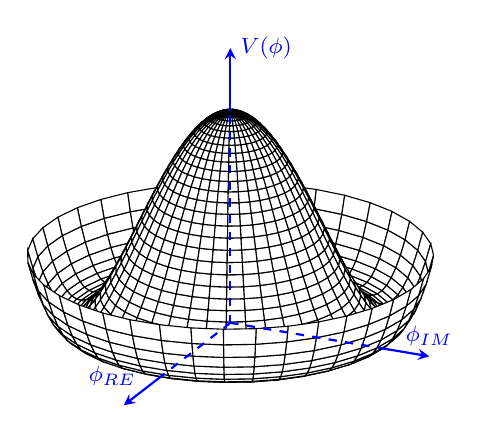
\begin{tikzpicture}

    \begin{axis}[
        %axis lines=center,
        %axis line style={->},
        hide axis,
        samples=40,
        domain=0:360,
        y domain=0:1.25,
        xtick=\empty,
        ytick=\empty,
        ztick=\empty
    ]
    \addplot3 [surf, shader=flat, draw=black, fill=white, z buffer=sort] ({sin(x)*y}, {cos(x)*y}, {(y^2-1)^2});

    \draw[blue,thick,dashed] (axis cs:0,0,0) -- (axis cs:1,0,0)
                %node[below,font=\footnotesize]{$\phi_{\text{IM}}$}
                ;
    \draw[blue,thick,-stealth] (axis cs:1,0,0) -- (axis cs:1.35,0,0)
                node[above,font=\footnotesize]{$\phi_{\text{IM}}$};

    \draw[blue,thick,dashed] (axis cs:0,0,0) -- (axis cs:0,-1,0)
                node[left=2mm,font=\footnotesize]{$\phi_{\text{RE}}$};
    \draw[blue,thick,-stealth] (axis cs:0,-1,0) -- (axis cs:0,-1.55,0)
                %node[right=1mm,font=\footnotesize]{$\phi_{\text{RE}}$}
                ;

    \draw[blue,thick,dashed] (axis cs:0,0,0) -- (axis cs:0,0,1)
                %node[left=2mm,font=\footnotesize]{$\phi_{\text{RE}}$}
                ;
    \draw[blue,thick,-stealth] (axis cs:0,0,1) -- (axis cs:0,0,1.3)
                node[right,font=\footnotesize]{$V(\phi)$};

    \end{axis}

\end{tikzpicture}
  \caption{
    The Higgs potential $V(\phi)$ of the complex scalar field singlet $\phi = \phi_1 + i \phi_2$, with a choice of $\mu^2 < 0$ leading to a continuous degeneracy in the true vacuum states. A false vacuum is present at the origin. The SM Higgs mechanism relies on a complex scalar doublet with a corresponding 5-dimensional potential.
  }
  \label{fig:higgs_potential}
\end{figure}
%

Consider gauge fields from the local $SU(2)_L \otimes U(1)_Y$ symmetry group discussed in \cref{sec:ew_sector} coupled to a complex scalar field $\phi = \phi(x)$. The scalar field $\phi$ transforms as a weak isospin doublet.
Omitting the kinetic term of the gauge fields, and writing $\phi^2 \equiv \phi^\dagger \phi$, the Lagrangain is
%
\begin{equation}\label{eq:sm_higgs_lagrangian}
  \mathcal{L}_{\textnormal{Higgs}} = 
  (D_\mu \phi)^\dagger (D^\mu \phi) - \left[ \mu^2 \phi^2 + \lambda \phi^4 \right],
\end{equation}
%
where the covariant derivative is given by
%
\begin{equation}\label{eq:sm_higgs_cov_derivative}
  D_\mu = \partial_\mu + i g A^a_\mu T^a + i g^\prime B_\mu ,
\end{equation}
%
and $T^a$ are the generators of $SU(2)$.
The potential term $V(\phi)$ is made up of a quadratic and quartic term in the scalar field $\phi$, which contain an arbitrary parameter, respectively $\lambda$ and $\mu$.
The quartic term gives the field self-interaction, and cannot be negative as this would lead to a potential that was unbounded from below.
The quadratic term can be positive or negative.
In the case where the quadratic term is positive, it is interpreted as a mass term for the scalar field
By choosing $\mu^2 < 0$ the field becomes unphysical due to its negative mass.
In order to obtain a physical interpretation of the Lagrangain in \cref{eq:sm_higgs_lagrangian} for the case where $\mu^2 < 0$, the field $\phi$ is expanded around the vacuum state.
The vacuum expectation value (VEV) is expected value of the field $\phi$ which minimises the potential $V(\phi)$ (equivalently the expected value of the field operator $\phi$ when the system is in a vacuum state, $|\langle{\phi}\rangle_0|^2 \equiv |\bra{0} \phi \ket{0}|^2 \equiv \vev{\phi}$).
%It is worth mentioning explicitly at this point that each base operator $\phi_i$ explicitly defines its own vev $\vev{\phi_i}$
Minimising the potential gives a VEV of
%
\begin{equation}\label{eq:higgs_vev}
  \vev{\phi} = -\mu^2 / \lambda = v^2 .
\end{equation}
%
Due to the shape of the potential in \cref{fig:higgs_potential}, there is degeneracy in the direction that the complex doublet $\phi$ points.
As all the different vacuum states minimise the potential and therefore yield identical physics, so we can arbitrarily choose the state to lie along the second component of the doublet.
Application of \cref{eq:charge_operator} shows this choice is manifestly invariant under, unbroken subgroup under which the ground state is invariant is $U(1)_Q$, generated by $Q$.
%Different vacuum states are traversed by moving in flat directions of the potential.
%Particles corresponding to fluctuations of the field along the flat directions in the potential are massless as they don't cost energy to attain.

% MORE ON PHYSICAL PARTICLE INTERP AND FIELD SUBSTITUITON
%For a field to be able to have the standard particle interpretation, it must be linear in creation and annihilation operators. Such a field has a vanishing vacuum expectation value. As such, fields with nonvanishing VEV cannot correspond to particles. The new field H has vanishing VEV
%  Now considering fluctuations (particle content) around this vacuum we obtain $\phi(\mathrm{x}) = v + f(\mathrm{x})$ as the sum of the vacuum contribution and scalar particle fluctuations. In effect, this is a field substitution, where the new field has the property $\vev{f} = 0$ (i.e $f = 0$ minimises the potential $V(\phi)$).
% This is the motivation behind the field substitution in equation (4.3), where the newly introduced
%field has a vanishing VEV by construction. Note that the original field remains massless, whereas the newly
%introduced field (corresponding to a physical particle) gains mass.


Adding the particle content back to the theory by expanding the field around the vacuum state, and making a transformation to the unitary gauge to remove unphysical would\nobreakdash-be Nambu-Goldstone modes (which arise in the context of global symmetries \cite{PhysRev.117.648,Goldstone1961FieldTW}) yields
% adding particle content is performing a field substitution
%transformation to the unitary gauge to regain physical interpretation
%
\begin{equation}
  \phi = 
  \frac{1}{\sqrt{2}}
  \begin{pmatrix}
    0 \\ v + H
  \end{pmatrix} ,
\end{equation}
%
Where $H$ is a real scalar field, the ``true vacuum'' Higgs field.
Substituting this into \cref{eq:sm_higgs_lagrangian} and identifying physical fields as quadratic terms of linear combinations, one can write the physical fields $W_\mu^\pm$, $Z_\mu$ and $A_\mu$ in terms of the original fields $A^a_\mu$ and $B_\mu$.
%The physical fields are the natural mass eigenstates that yield quadratic terms of the form $m^2 \chi^\mu\chi_\mu$.
This gives
%
\begin{equation}\label{eq:ew_physical_unphysical_fields}
  W_\mu^\pm = 
  \frac{1}{\sqrt{2}} (A^1_\mu \mp i A^2_\mu)
  \quad
  \begin{pmatrix}
    A_\mu \\ Z_\mu
  \end{pmatrix} =
  \begin{pmatrix}
      \cos\theta_W &  \sin\theta_W \\ 
    - \sin\theta_W &  \cos\theta_W
  \end{pmatrix}
  \begin{pmatrix}
    B_\mu \\ A^3_\mu 
  \end{pmatrix} .
\end{equation}
%
where $\theta_W$ is the weak mixing angle defined by 
%
\begin{equation}\label{eq:ew_coupling_weak_mixing_angle}
  \cos\theta_W = \frac{g}{\sqrt{g^2 + {g^\prime}^2}} .
\end{equation}
%
The corresponding masses of the now massive vector bosons can be read off as 
%
\begin{equation}
  m_W = \frac{1}{2} g v
  \quad
  m_Z = \frac{m_W}{\cos\theta_W} , %v^2 = \frac{m_W^2}{\cos^2\theta_W} .
\end{equation}
%
while the photon remains massless.
The Higgs mass is $m_H = v \sqrt{\lambda} = \mu$.

This is the Higgs mechanism.
It maintains the renormalisability and unitary of the SM whilst allowing the weak vector bosons to acquire mass.
In summary, an unphysical complex scalar field $\phi$ with a nonzero VEV leads to spontaneous symmetry breaking from the full SM symmetry group $SU(3)_C \otimes SU(2)_L \otimes U(1)_Y$ to $SU(3)_C \otimes U(1)_\gamma$.
Due to the non-Abelian symmetry breaking, would\nobreakdash-be massless Nambu-Goldstone modes, which arise after expansion around the true vacuum state, are exactly cancelled out by making a local gauge transformation to the unitary gauge, and instead are absorbed by the vector bosons, allowing them to acquire mass.

This sector of the SM contains four fundamental parameters that must be taken from experiment.
These can be specified by the Lagrangian parameters $g$, $g^\prime$, $v$ and $\lambda$ or the physically measurable parameters $m_Z$, $\sin\theta_W$, $m_H$ and $e$.
In the local neighbourhood around the true vacuum, the macroscopic symmetry of the system is not realised, and therefore the physical particles do not obey the original symmetry. 
However, information about the symmetry is retained through some additional constraints on the particles and their interactions.
Prior to symmetry breaking, the potential contained two terms and two constants. After symmetry breaking we have three terms but still only two constants that relate these terms. This is the vestige of the original symmetry. %Because we have related $\mu$, $\lambda$ and $v$, when these would be three independent parameters if we had no symmetry.
%Note critically that symmetry places conditions on the two interaction terms, which are related to each other through the constants $\lambda$ and $v$. As $v$ already parameterises the mass of the field $f$, these two interaction terms are described by only one additional constant $\lambda$, when in general these terms could have their own independent coupling.

Spontaneous symmetry breaking has taken us from $SU(2)_L \times U(1)_Y \rightarrow U(1)_{\gamma}$.
Three broken generators of the symmetry group $U(2) = SU(2) \otimes U(1)$ have been absorbed into the definition of the physical weak vector bosons, giving them mass.
The same methodology can be used to generate the fermion masses, as shown in the next section. 





\subsection{Fermionic Yukawa Coupling}\label{sec:higgs_yukawa_coupling}

Adding the masses of the fermions by hand breaks the gauge invariance of the theory.
%the necessity for fermion masses being generated in this way is different from that of the vector bosons, which cannot have locally invariant bilinear field terms in the Lagrangian. For the fermions, we cannot write a mass term due to the 
\begin{comment}
The reason is as follows: consider the standard \textbf{Dirac mass term} that we use to give mass to particles 
%
\begin{equation}\label{dirac mass term}
    m \overline{\psi} \psi = m (\overline{\psi}_L + \overline{\psi}_R) ({\psi}_L + {\psi}_R) = m({\overline{\psi}}_L \psi_R + \overline{\psi}_R \psi_L) ,
\end{equation}
%
where the $\overline{\psi}_L \psi_L$ and $\overline{\psi}_R \psi_R$ vanish due to the anticommutation of $\gamma^5 \gamma^0 = - \gamma^0 \gamma^5$, and the fact tat $P_L P_R = P_R P_L = 0$. Concretely, we have
%
\begin{equation}\label{same chirality spinor bilinear vanishes}
    \overline{\psi}_L \psi_L = \psi^\dagger P_L \gamma^0 P_L \psi = \overline{\psi} P_R P_L \psi = 0.
\end{equation}
%
Note that $\overline{\psi}_L = \overline{\psi_L}$. Now, \cref{dirac mass term} is note invariant under electroweak gauge transformations as the LH spinors transform under $SU(2)_L$ while RH spinors transform under $U(1)_Y$ (i.e. we could do an $SU(2)$ transformation that would affect $\psi_L$ but not $\psi_R$ which is clearly not invariant). 
\end{comment}
Instead, we can use a Yukawa coupling of the fermion fields with the Higgs field in order to generate mass terms after spontaneous electroweak symmetry breakdown \cite{Weinberg:1967tq}.
In this way, the fermion masses are determined by the respective couplings to the Higgs field, and the VEV of the Higgs field itself, which sets the basic mass scale of the theory.

If the $T = 1/2$ doublet $\phi$ has weak hypercharge $Y = 1/2$, then there is a unique renormalisable and gauge invariant coupling given by
%
\begin{equation}\label{eq:yukawa_coupling}
  \mathcal{L}_{\textnormal{Yukawa}} = 
  - G_f (\overline{\psi}_L \phi \psi_R + \overline{\psi}_R \phi \psi_L)
\end{equation}
%


The Yukawa terms mix quarks of different generations. The indices on the $\Lambda$ matrix stand for the generations, and the elements of $\Lambda$ are complex valued.

The physical particles are detected in their mass eigenstates (but transform under $SU(2)$ according to their weak eigenstates). In other words, the physical particles diagonalise the mass matrix. It therefore makes sense to work in a basis that diagonalises the mass matrix. These are the mass eigenstates, as opposed to the weak eigenstates. Quark mixing can be expressed using the CKM matrix.
%
\begin{equation}
    \begin{pmatrix}
        \tilde{d} \\ \tilde{s} \\ \tilde{b} 
    \end{pmatrix}
    = \begin{pmatrix}
        V_{ud} & V_{us} & V_{ub} \\  
        V_{cd} & V_{cs} & V_{cb} \\  
        V_{td} & V_{ts} & V_{tb} 
    \end{pmatrix}
    \begin{pmatrix}
        {d} \\ {s} \\ {b} 
    \end{pmatrix}
\end{equation}
%
The CKM matrix is a result of the transformation between mass and gauge eigenstates of the quarks. It is a unitary matrix which contains information on the strength of flavour-changing weak decays. The $\tilde{q}$ represent gauge or weak eigenstates, whereas $q$ represent mass eigenstates. The size of the elements $|V_{pq}|^2$ measures the probability of a transition between states $p$ and $n$.

We start with the most general form of the coupling of the $T = 1/2$, $Y=1/2$ Higgs field $\phi$ to the quark fields. From $\phi$ we can form a conjugate field $\phi^c$ which transforms under $SU(2) \otimes U(1)_Y$ as a doublet with $Y = -1/2$,
%
\begin{equation}\label{phi c field definition}
    \phi^c = i \sigma_2 \phi^* = 
    \begin{pmatrix}
    0 & 1 \\ -1 & 0
    \end{pmatrix} 
    \begin{pmatrix}
    {\phi_1}^\dagger \\ {\phi_2}^\dagger
    \end{pmatrix} = \begin{pmatrix}
    {\phi_2}^\dagger \\ -{\phi_1}^\dagger
    \end{pmatrix} .
\end{equation}
%
We can see (???) that $\phi^c$ transforms under $SU(2)$ in the same way as $\phi$. The ground state of this conjugate field is 
%
\begin{equation}
    {\phi_0}^c = \frac{1}{\sqrt{2}} \begin{pmatrix} v \\ 0 \end{pmatrix} .
\end{equation}
%
The general gauge invariant expression for the coupling of the Higgs field to the quark fields is then of the form (???)
%
\begin{equation}\label{quark mass term}
    \mathcal{L}_{\phi, \text{quarks}} = - \sqrt{2} \left[ \overline{L}_N f^-_{NM} \phi R_{M-} +
    \overline{L}_N f^+_{NM} \phi^c R_{M+} + \text{h.c.}
    \right] ,
\end{equation}
%


\subsection{Higgs Phenomenology}

\begin{itemize}
  \item Production mechanisms
  \item Decay modes
  \item Relevance to analysis Vhbb
\end{itemize}


%In 2015, 
%Run 2
%the LHC started to collide protons at a centre of mass energy of \come{13}.
%The cross sections for the SM production modes increase by a factor of approximately two to four, depending
%on the process, and the anticipated integrated luminosity for Run 2 which is scheduled to end in 2018 is
%of the order of 120 fb−1
%per experiment. Such a dataset will allow ATLAS and CMS to reduce the current
%experimental uncertainties significantly, motivating the need for improved theoretical predictions.

\begin{figure}[!htbp]
  \centering
  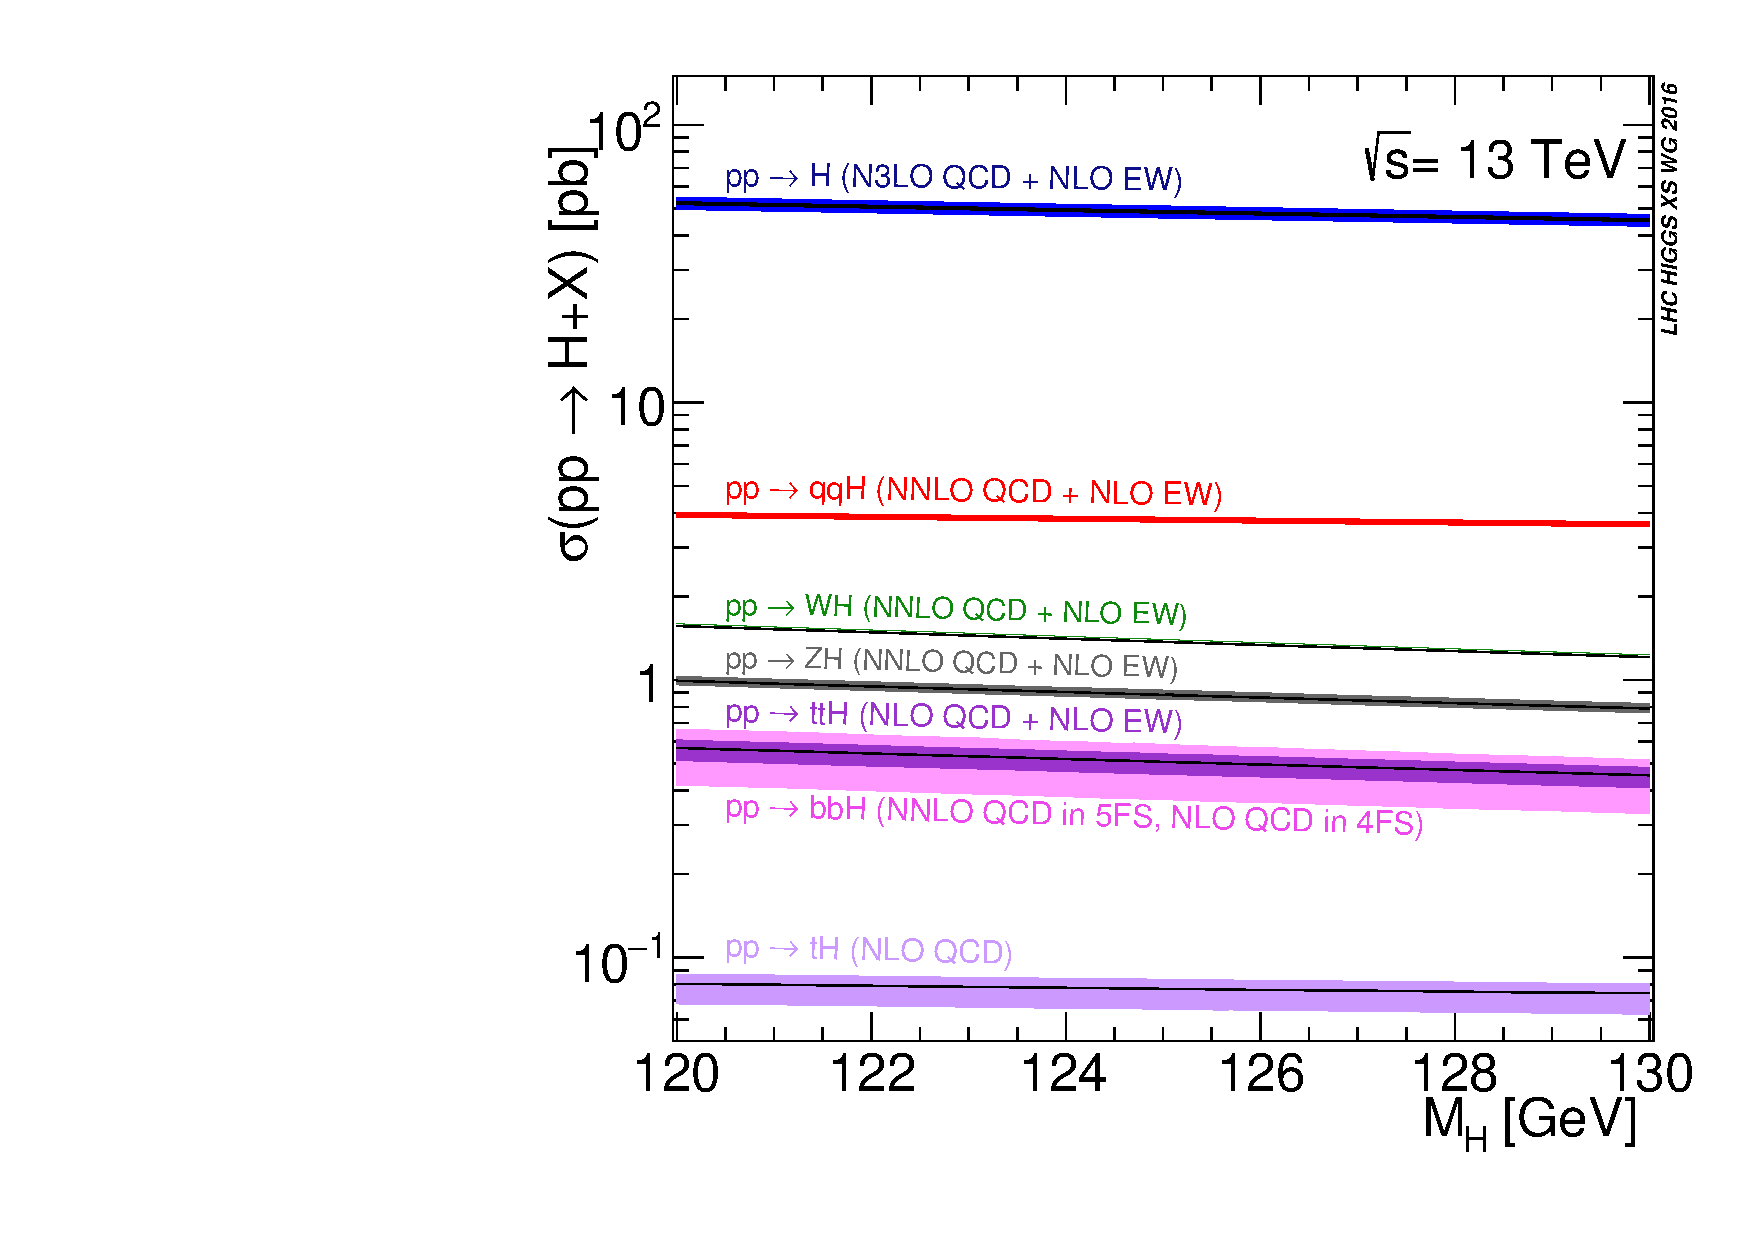
\includegraphics[width=0.5\linewidth]{chapters/1.theory/figs/plot_13tev_H_sqrt.pdf}
  \caption{Higgs production cross sections at $\sqrt{s} = \SI{13}{\TeV}$ \cite{deFlorian:2016spz}.}
  \label{fig:higgs_production_xs}
\end{figure}

\begin{figure}[!htbp]
  \centering
  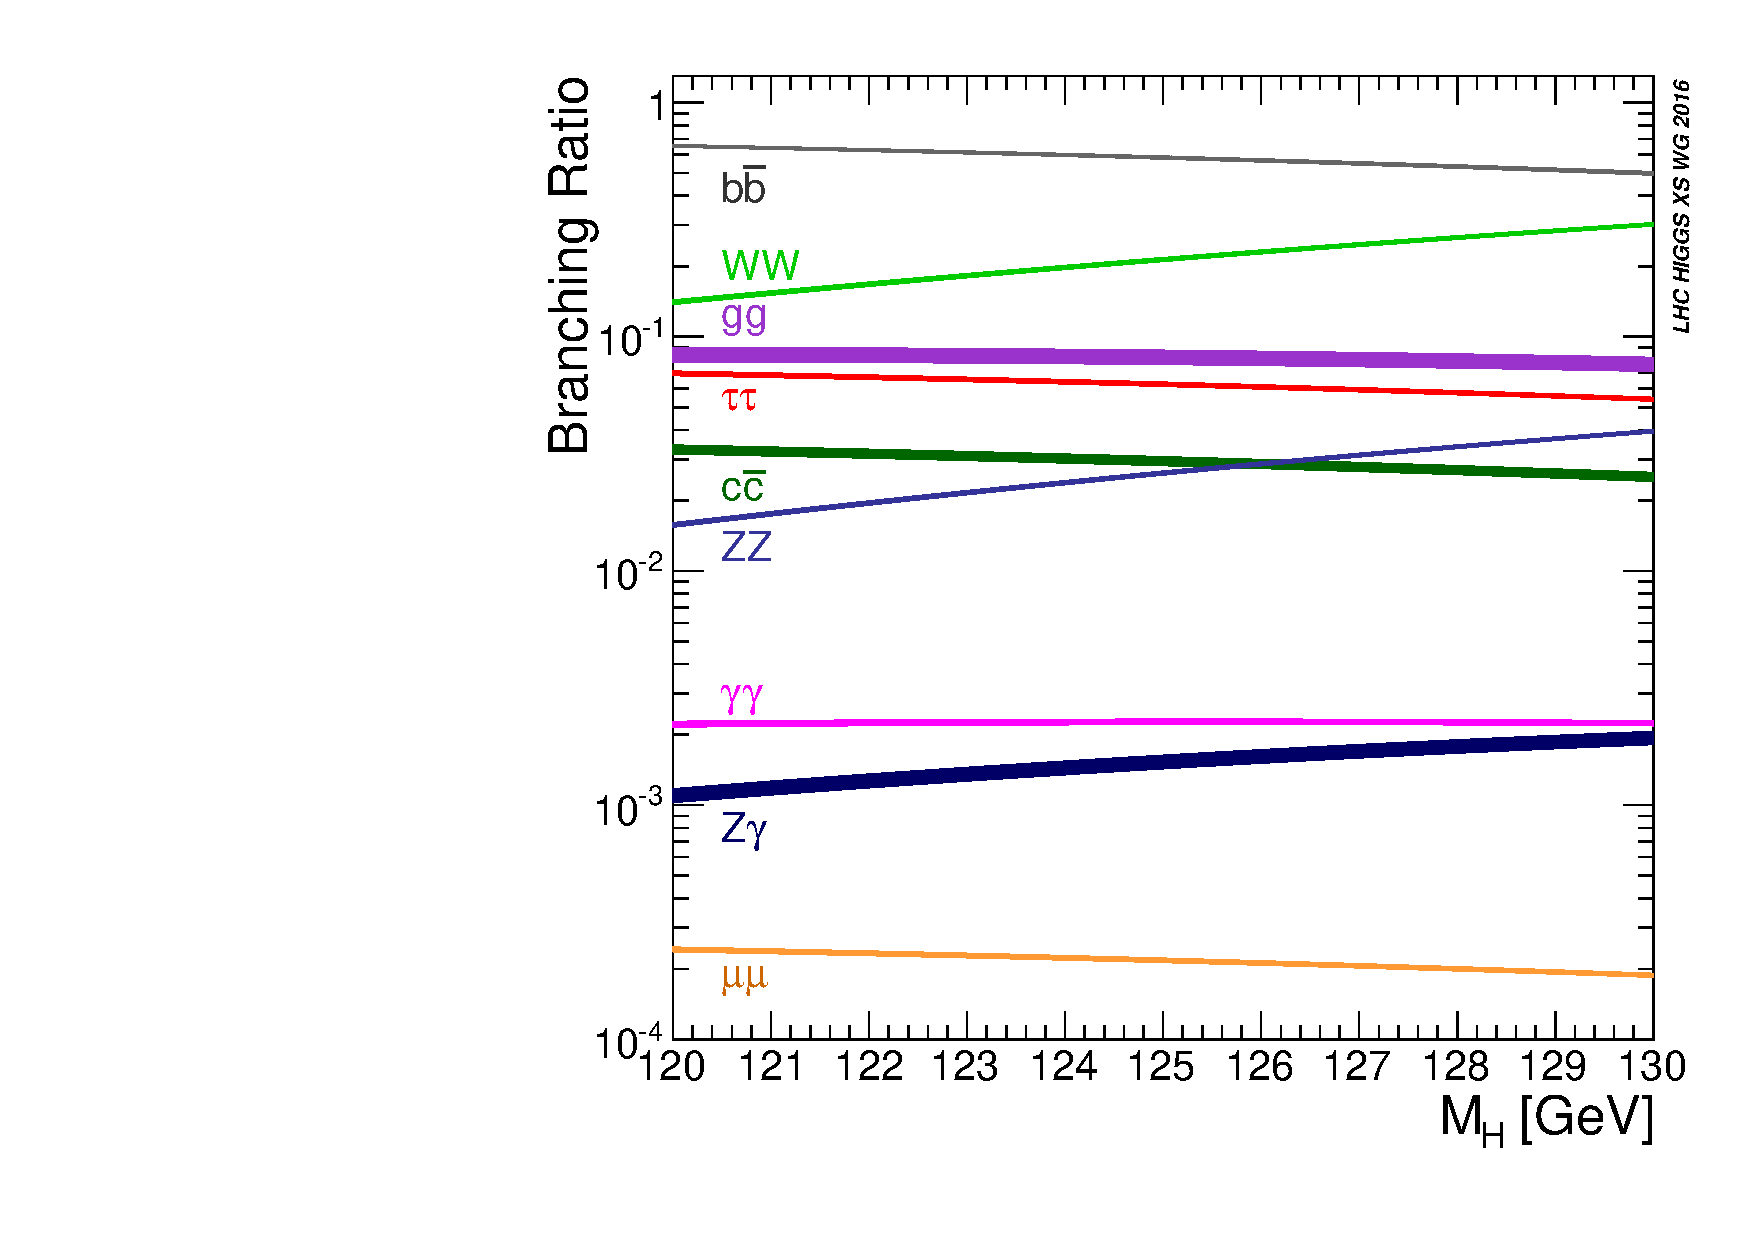
\includegraphics[width=0.5\linewidth]{chapters/1.theory/figs/SMHiggsBR.YR4-square.pdf}
  \caption{Higgs branch ratios at $\sqrt{s} = \SI{13}{\TeV}$ \cite{deFlorian:2016spz}.}
  \label{fig:higgs_br}
\end{figure}
